\subsection{Meldeprint}
Die Software des Meldeprints ist in drei Bereiche unterteilt: Initialisierung, Interrupt, Statusüberwachung. Beinahe die ganze Überwachung der Module kann im Bereich ''Statusüberwachung'' abgehandelt werden. Die anderen beiden dienen zum einen für die Anzeige und die Initialisierung, zum anderen für die Aktualisierung der eingehenden Daten.

\begin{figure}[htbp] 
  \centering
     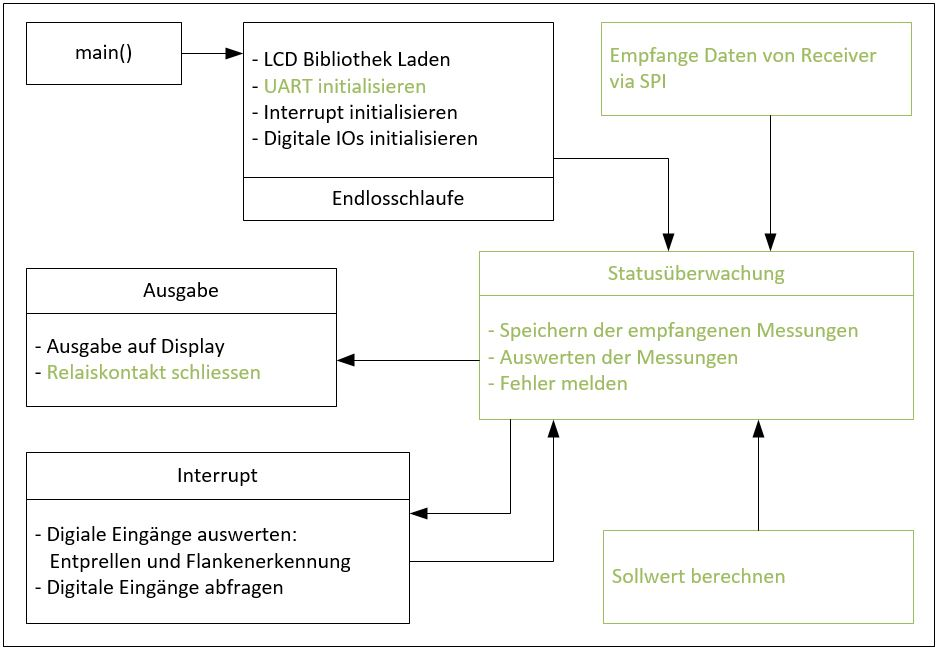
\includegraphics[width=0.8\textwidth]{graphics/reportboard-software-river}
  \caption{Visualisierung Softwarekonzept}
  \label{fig:reportboard-software-river}
\end{figure}

Wie die Bereiche der Software zusammenarbeiten ist in Abbildung \ref{fig:reportboard-software-river} gut ersichtlich. In der Initialisierung werden als Erstes die Hardwarekomponenten  und Interrupts initialisiert, anschliessend wird die Endlosschlaufe im Hauptprogramm aufgerufen.\\
Der Timer-Interrupt hat zwei Aufgaben. Er entprellt alle 15$\mu$s die digitalen Eingänge und führt eine Flankendetektion durch. Das wird gebraucht für den Encoder, damit kann der Benutzer den Cursor auf dem Display punktgenau einstellen und den Encoder drücken ohne dass er prellt. Vom Receiver über SPI übermittelte Daten lösen einen Interrupt aus, der die Datenpakete im Hauptprogramm weiterverarbeitet.\\
Die eingegangenen Daten der gemessenen Spannungen werden zusammen mit der Identifikationsnummer von der Routine ''Statusüberwachung'' in ein Array gespeichert und mit dem von der Routine ''Sollwert'' berechneten Durchschnitt verglichen. Der Sollwert entspricht dem arithmetischen Mittelwert der Spannungen dieses einen Strings. Hat eine Modulspannung eine bestimmte Abweichung wird dieses Modul vorgemerkt. Falls nach einer weiteren Messung die Spannung desselben Moduls gleichviel vom Mittelwert abweicht, wird ein Fehler gemeldet. Die Identifikationsnummer wird auf dem Display angezeigt.\\
Der ganze Prozess vom Start des Meldeprints bis zur Fehlermeldung werden hier weiter vertieft behandelt. Dabei ist anzumerken, dass die beschriebenen Prozesse nicht programmiert und getestet werden konnten.

\subsubsection{Inbetriebnahme}
Wird die Software gestartet beginnt die Initialisierung der Peripheriegeräte. In diesem Abschnitt wird der Display und die Kommunikation mit dem Receiver initialisiert. Ist dieser Vorgang abgeschlossen ruft das Hauptprogramm die Routine ''Statusüberwachung''. Der Meldeprint ist nun betriebsbereit und reagiert sobald eine Eingabe vom Benutzer \ref{Benutzerinterface} getätigt wird oder der Interrupt ein eingehendes Datenpaket registriert. Die Datenpakete des Sensorprints würden nun erkannt und im Hauptprogramm in ein Registerarray gespeichert werden.

\subsubsection{Receiver}
Der Receiver detektiert über einen Ferrit-Kern über der DC-Leitung des Strings die Signale des Sensorprints. Die Datenpakete werden mit der Identifikationsnummer und der Prüfsumme an den Mikrocontroller weitergeleitet. Diese Kommunikation soll auf SPI basieren. Die Checksum soll ausgewertet werden. Detektiert diese keine Übertragungsfehler, sollen die Informationen weiter verarbeitet werden. Ansonsten wird eine weitere Übertragung derjenigen Sensorplatine abgewartet. \\
Die Kommunikation über die DC-Leitung zwischen Sensorprint und Meldeprint ist unidirektional. Ist der Meldeprint eingeschaltet und die Initialisierung des Receivers abgeschlossen, können laufend vom Sensorprint gesendete Datenpakete empfangen werden. Der im Hauptprogramm zuvor initialisierte Interrupt registriert die empfangenen Daten vom Receiver und verarbeitet diese weiter.

\subsubsection{Fehlererkennung}
Die Fehlererkennung spielt eine zentrale Rolle im gesamten Überwachungssystem von Sensor- und Meldeprint. Eine übersichtliche und einfache Lösung ist die Fehlererkennung mithilfe des arithmetischen Mittels zusammen mit einer Identifikationsnummer.\\
Die Variante will die gemittelten Spannungswerte, die jede Sensorplatine liefert, nochmals über alle Module des Strings mitteln. Damit kann die Standardabweichung berechnet werden.\todo{Haben wir eine Rechnung für Standardabweichung} Ist die Abweichung eines Spannungswerts mehr als 20 Prozent von der Standardabweichung, wird dieses Solarmodul vorgemerkt. Weicht der Spannungswert des vorgemerkten Moduls nach der nächsten Stunde noch immer stark vom Mittelwert ab, wird eine Fehlermeldung ausgegeben. Eine dem vorgemerkten Spannungswert hinterlegte Identifikationsnummer ermöglicht das exakte Ermitteln des fehlerhaften Moduls und es im String zu finden.

\begin{figure}[htbp] 
  \centering
     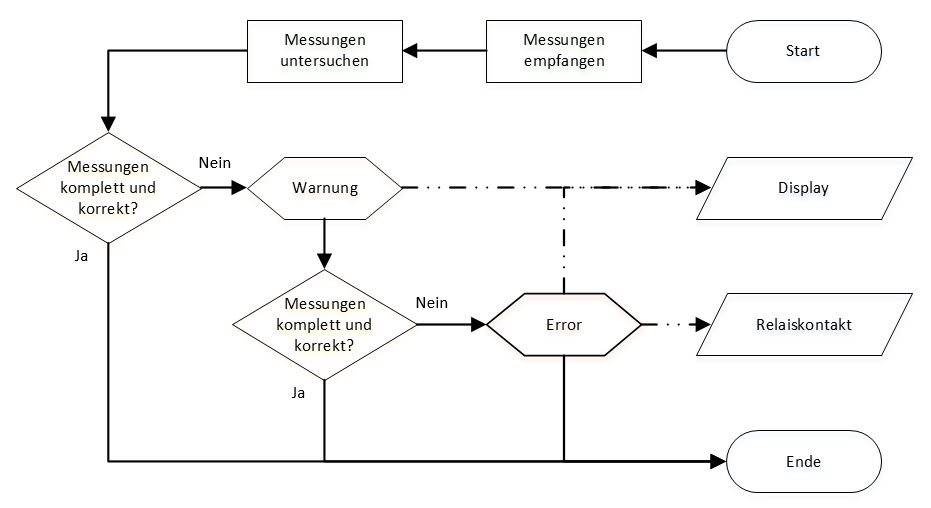
\includegraphics[width=0.8\textwidth]{graphics/error-warning-scheme}
  \caption{Prozess zur Fehlererkennung}
  \label{fig:error-warning-scheme}
\end{figure}


Dieser Prozess wiederholt sich stündlich und ist in Abbildung \ref{fig:error-warning-scheme} sichtbar.

\subsubsection{Fehlermeldung}
Wird ein defektes oder beschmutztes Modul detektiert wird eine entsprechende Fehlermeldung auf dem Display ausgegeben. Zusätzlich zu dieser Information sollen die Identifikationsnummer und der allfällige Name des Panels ausgegeben werden.\\
Ist der allgemeine Mittelwert über zwei Stunden tief, wird darauf geschlossen, dass Dunkelheit herrscht. In dieser Situation wird keine Fehlermeldung ausgegeben.

\subsubsection{Benutzerinterface}
Das Menü und der Drehgeber bilden zusammen eine einfache Schnittstelle zwischen Mensch und Maschine. Für das auswählen eines Eintrages wird der Encoder gedrückt. Für den umgekehrten Weg ist in jedem Untermenü und in jedem Eintrag eine Zurück-Funktion. Das Menü ist in zwei Ebenen unterteilt welche in Abbildung \ref{fig:structure-menu} dargestellt ist.
\newpage
\begin{figure}[htbp] 
  \centering
     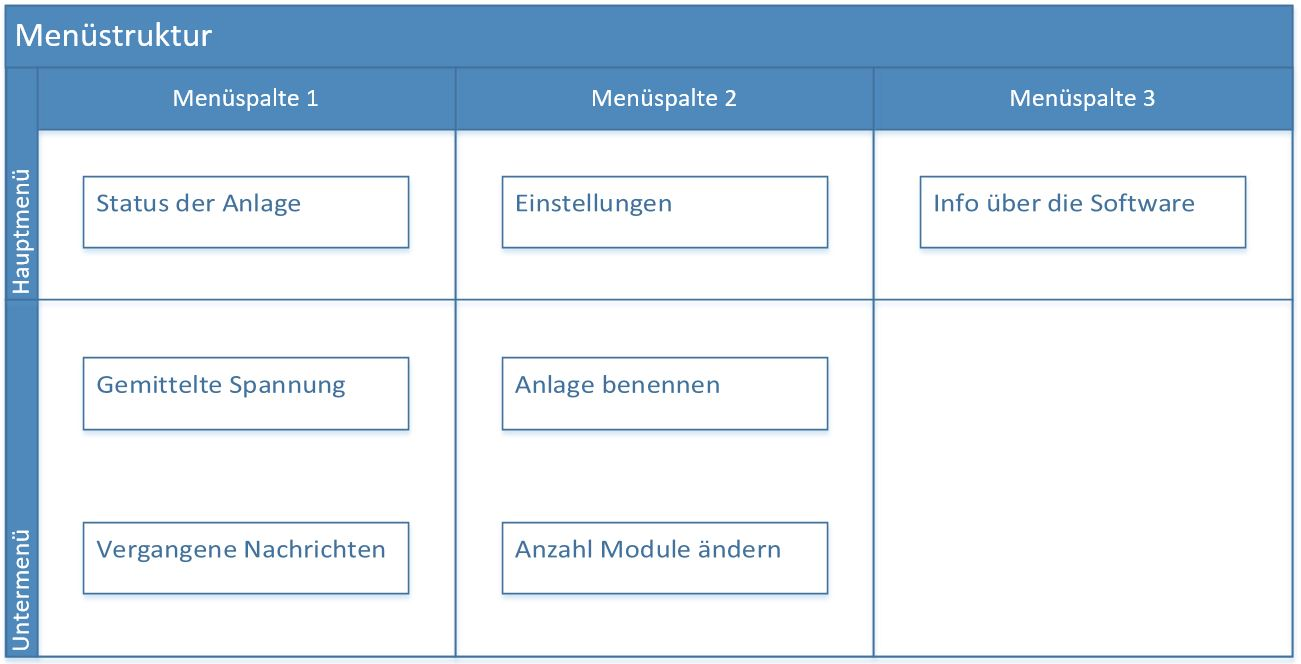
\includegraphics[width=0.8\textwidth]{graphics/structure-menu}
  \caption{Menüstruktur}
  \label{fig:structure-menu}
\end{figure}

In der Hauptmenü-Zeile befinden sich die drei Einträge: ''Status der Anlage'', ''Einstellungen'' und ''Info über die Software'', die in Abbildung \ref{fig:structure-menu} zu sehen sind.\\
Im ersten Untermenü kann der Benutzer zwischen zwei Informationen wählen: abfragen der aktuellen gemittelten Spannung und nachschauen aller Nachrichten seit dem letzten Zurücksetzen des Meldeprints.\\
Im zweiten Untermenü kann der Benutzer Einstellungen vornehmen. Er hat die Möglichkeit dem Meldeprint einen Namen zu geben. Weiter muss die Menge der überwachten Module angegeben werden.\\
Im dritten Untermenü werden Informationen zur aktuellen Software und dem Hersteller angezeigt.\\